\documentclass[aspectratio=169,11pt]{beamer}
\usetheme{metropolis}
\usepackage{tikz}
\usetikzlibrary{arrows.meta,positioning,decorations.pathmorphing,calc,shapes.geometric,decorations.pathreplacing,patterns}
\usepackage{pgfplots}
\pgfplotsset{compat=1.18}
\usepackage{booktabs}
\usepackage{xcolor}
\usepackage{amsmath}
\usepackage{graphicx}
\graphicspath{{figures/}}

\definecolor{evidence}{HTML}{2196F3}
\definecolor{choice}{HTML}{E91E63}
\definecolor{geometry}{HTML}{4CAF50}
\definecolor{causal}{HTML}{FF9800}
\definecolor{neutral}{HTML}{9E9E9E}
\definecolor{pass}{HTML}{4CAF50}
\definecolor{fail}{HTML}{F44336}
\definecolor{partial}{HTML}{FF9800}
\definecolor{dimhigh}{HTML}{D32F2F}
\definecolor{dimlow}{HTML}{1565C0}
\definecolor{bg}{HTML}{FAFAFA}

\title{Geometric Structure in Neural Population Codes}
\subtitle{A tool-comparison framework for causal neural geometry\\[0.3em]
{\small Exploratory results on Steinmetz 2019}}
\author{Elliot Tower}
\date{2026}
\institute{}

\begin{document}

\maketitle

%% ============================================================
%% PART 1: SETUP — accessible framing
%% ============================================================

%% --- SLIDE: The basic question ---
\begin{frame}{The question}

When a population of neurons fires together during a decision, does the \textbf{shape} of that activity matter---or just the individual firing rates?

\vspace{1em}

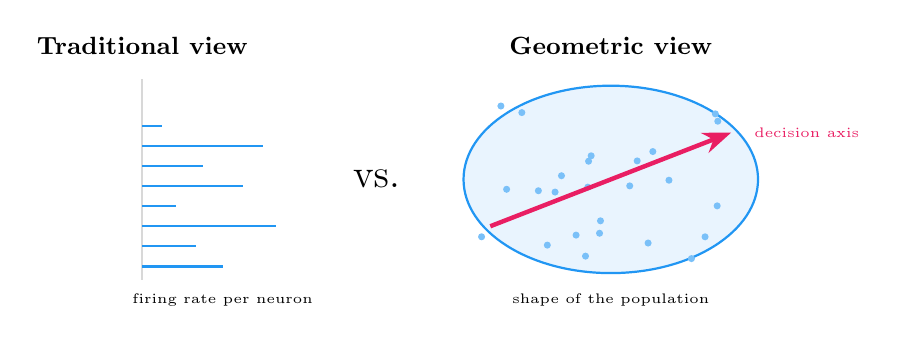
\begin{tikzpicture}[scale=0.85]
  % Left: single neuron view
  \node[font=\small\bfseries] at (0,3.5) {Traditional view};
  \draw[neutral!40,thick] (0,0) -- (0,3);
  \foreach \y/\h in {0.2/1.2, 0.5/0.8, 0.8/2.0, 1.1/0.5, 1.4/1.5, 1.7/0.9, 2.0/1.8, 2.3/0.3} {
    \draw[evidence,thick] (0,\y) -- (\h,\y);
  }
  \node[font=\tiny] at (1.2,-0.3) {firing rate per neuron};

  % Arrow
  \node[font=\Large] at (3.5,1.5) {vs.};

  % Right: population geometry view
  \node[font=\small\bfseries] at (7,3.5) {Geometric view};
  \fill[evidence!10] (7,1.5) ellipse (2.2 and 1.4);
  \draw[evidence,thick] (7,1.5) ellipse (2.2 and 1.4);
  % Points = trials
  \foreach \i in {1,...,25} {
    \pgfmathsetmacro{\rx}{2.0*rand}
    \pgfmathsetmacro{\ry}{1.2*rand}
    \fill[evidence!60] (7+\rx,1.5+\ry) circle (1.5pt);
  }
  \draw[choice,ultra thick,-{Stealth}] (5.2,0.8) -- (8.8,2.2);
  \node[choice,font=\tiny,anchor=west] at (9,2.2) {decision axis};
  \node[font=\tiny] at (7,-0.3) {shape of the population};
\end{tikzpicture}

\vspace{0.5em}
We tested this on real brain recordings, using multiple tools, with causal interventions and validity checks.
\end{frame}

%% --- SLIDE: What is neural geometry? ---
\begin{frame}{What is ``neural geometry''?}
\begin{columns}[T]
\begin{column}{0.55\textwidth}
{\small Each \textbf{trial} produces a pattern of activity across a collection of neurons. Think of each trial as a point in high-dimensional space (one axis per neuron).}

\vspace{0.3em}
{\small ``Geometry'' = what \textbf{shape} do those points form?}
\begin{itemize}\setlength\itemsep{0pt}
  \item {\small Cluster into groups? (categories)}
  \item {\small Spread along a line? (gradient)}
  \item {\small Form a loop? (periodic variable)}
  \item {\small Lie on a flat sheet or curved surface?}
\end{itemize}

\vspace{0.3em}
{\small The shape constrains what information the brain can extract downstream.}
\end{column}
\begin{column}{0.42\textwidth}
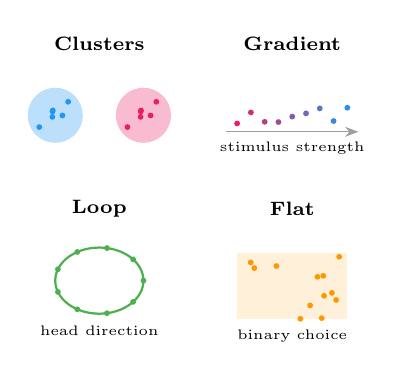
\begin{tikzpicture}[scale=0.7]
  % Example 1: clusters
  \node[font=\scriptsize\bfseries] at (0,5.0) {Clusters};
  \fill[evidence!30] (-0.8,3.7) circle (0.5);
  \fill[choice!30] (0.8,3.7) circle (0.5);
  \foreach \i in {1,...,6} {
    \pgfmathsetmacro{\rx}{0.3*rand}
    \pgfmathsetmacro{\ry}{0.3*rand}
    \fill[evidence] (-0.8+\rx,3.7+\ry) circle (1.5pt);
    \fill[choice] (0.8+\rx,3.7+\ry) circle (1.5pt);
  }

  % Example 2: line/gradient
  \node[font=\scriptsize\bfseries] at (3.5,5.0) {Gradient};
  \foreach \i in {0,...,8} {
    \pgfmathsetmacro{\x}{2.5+\i*0.25}
    \pgfmathsetmacro{\c}{\i*12}
    \fill[evidence!\c!choice] (\x,3.7+0.15*rand) circle (1.5pt);
  }
  \draw[neutral,thin,-{Stealth}] (2.3,3.4) -- (4.7,3.4);
  \node[font=\tiny] at (3.5,3.1) {stimulus strength};

  % Example 3: loop
  \node[font=\scriptsize\bfseries] at (0,2.0) {Loop};
  \draw[geometry,thick] (0,0.7) ellipse (0.8 and 0.6);
  \foreach \a in {0,40,...,320} {
    \fill[geometry] ({0.8*cos(\a)},{0.7+0.6*sin(\a)}) circle (1.5pt);
  }
  \node[font=\tiny] at (0,-0.2) {head direction};

  % Example 4: flat sheet
  \node[font=\scriptsize\bfseries] at (3.5,2.0) {Flat};
  \fill[causal!15] (2.5,0) -- (4.5,0) -- (4.5,1.2) -- (2.5,1.2) -- cycle;
  \foreach \i in {1,...,12} {
    \pgfmathsetmacro{\rx}{2.5+2*rnd}
    \pgfmathsetmacro{\ry}{1.2*rnd}
    \fill[causal] (\rx,\ry) circle (1.5pt);
  }
  \node[font=\tiny] at (3.5,-0.3) {binary choice};
\end{tikzpicture}
\end{column}
\end{columns}
\end{frame}

%% --- SLIDE: Two tools for measuring geometry ---
\begin{frame}{Two tools for measuring geometry}
\begin{columns}[T]
\begin{column}{0.48\textwidth}
\centering
\textbf{\textcolor{dimlow}{CKA (linear)}}

\vspace{0.2em}
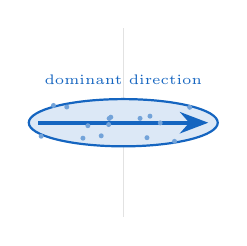
\begin{tikzpicture}[scale=0.6]
  \draw[neutral!30] (-2,0) -- (2,0);
  \draw[neutral!30] (0,-2) -- (0,2);
  \fill[dimlow!15] (0,0) ellipse (2 and 0.5);
  \draw[dimlow,thick] (0,0) ellipse (2 and 0.5);
  \draw[dimlow,ultra thick,-{Stealth}] (-1.8,0) -- (1.8,0);
  \node[dimlow,font=\tiny,above] at (0,0.6) {dominant direction};
  \foreach \i in {1,...,15} {
    \pgfmathsetmacro{\x}{1.8*rand}
    \pgfmathsetmacro{\y}{0.4*rand}
    \fill[dimlow!60] (\x,\y) circle (1.5pt);
  }
\end{tikzpicture}

\vspace{0.2em}
{\small Compares the \textbf{main axis} of variation.}

{\small ``Do the data stretch the same way?''}

{\small Best for low-dimensional data.}
\end{column}
\begin{column}{0.48\textwidth}
\centering
\textbf{\textcolor{dimhigh}{Procrustes (manifold)}}

\vspace{0.2em}
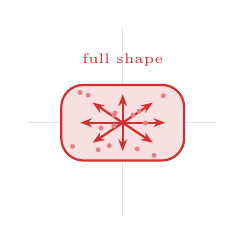
\begin{tikzpicture}[scale=0.6]
  \draw[neutral!30] (-2,0) -- (2,0);
  \draw[neutral!30] (0,-2) -- (0,2);
  \fill[dimhigh!15,rounded corners=8pt] (-1.3,-0.8) rectangle (1.3,0.8);
  \draw[dimhigh,thick,rounded corners=8pt] (-1.3,-0.8) rectangle (1.3,0.8);
  \foreach \a in {0,45,...,315} {
    \draw[dimhigh,thick,-{Stealth[length=1.5mm]}] (0,0) -- ({0.9*cos(\a)},{0.6*sin(\a)});
  }
  \node[dimhigh,font=\tiny,above] at (0,1.0) {full shape};
  \foreach \i in {1,...,15} {
    \pgfmathsetmacro{\x}{1.1*rand}
    \pgfmathsetmacro{\y}{0.7*rand}
    \fill[dimhigh!60] (\x,\y) circle (1.5pt);
  }
\end{tikzpicture}

\vspace{0.2em}
{\small Compares the \textbf{full shape} via rotation + scaling.}

{\small ``Do the data form the same cloud?''}

{\small Best for high-dimensional data.}
\end{column}
\end{columns}

\vspace{0.3em}
\centering
{\small Most prior work treats these as interchangeable. \textbf{They are not.}}
\end{frame}

%% --- SLIDE: The data ---
\begin{frame}{The data: Steinmetz et al.\ 2019}
\begin{columns}[T]
\begin{column}{0.5\textwidth}
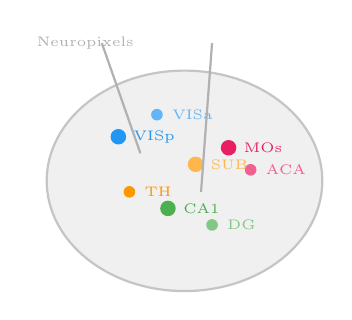
\begin{tikzpicture}[scale=0.7]
  \fill[neutral!15] (0,0) ellipse (2.5 and 2);
  \draw[neutral!60,thick] (0,0) ellipse (2.5 and 2);
  \fill[evidence] (-1.2,0.8) circle (4pt) node[right,font=\tiny,xshift=2pt] {VISp};
  \fill[evidence!70] (-0.5,1.2) circle (3pt) node[right,font=\tiny,xshift=2pt] {VISa};
  \fill[choice] (0.8,0.6) circle (4pt) node[right,font=\tiny,xshift=2pt] {MOs};
  \fill[choice!70] (1.2,0.2) circle (3pt) node[right,font=\tiny,xshift=2pt] {ACA};
  \fill[geometry] (-0.3,-0.5) circle (4pt) node[right,font=\tiny,xshift=2pt] {CA1};
  \fill[geometry!70] (0.5,-0.8) circle (3pt) node[right,font=\tiny,xshift=2pt] {DG};
  \fill[causal] (-1.0,-0.2) circle (3pt) node[right,font=\tiny,xshift=2pt] {TH};
  \fill[causal!70] (0.2,0.3) circle (4pt) node[right,font=\tiny,xshift=2pt] {SUB};
  \draw[neutral!80,thick] (-1.5,2.5) -- (-0.8,0.5);
  \draw[neutral!80,thick] (0.5,2.5) -- (0.3,-0.2);
  \node[font=\tiny,neutral!80] at (-1.8,2.5) {Neuropixels};
\end{tikzpicture}
\end{column}
\begin{column}{0.5\textwidth}
\begin{itemize}
  \item \textbf{39 sessions} from \textbf{10 mice}
  \item \textbf{73 brain regions} recorded simultaneously
  \item Neuropixels probes (${\sim}30{,}000$ neurons total; ${\sim}50$--$500$ per region per session)
  \item \textbf{Task:} visual discrimination \\
    {\small Two screens show visual noise at different contrasts. Mouse turns a wheel toward the higher-contrast side.}
  \item 1,316 pairwise region comparisons
\end{itemize}
\vspace{0.5em}
{\small \textcolor{neutral}{Steinmetz et al., Nature 2019}}
\end{column}
\end{columns}
\end{frame}

%% ============================================================
%% PART 2: FINDINGS — descriptive geometry
%% ============================================================
\section{What we found: the tools disagree}

%% --- SLIDE: Why they disagree — concrete example ---
\begin{frame}{Why CKA and Procrustes give opposite answers}
\begin{columns}[T]
\begin{column}{0.5\textwidth}
\centering
\textbf{\textcolor{dimlow}{Low-dimensional region (VISp-type)}}

\vspace{0.3em}
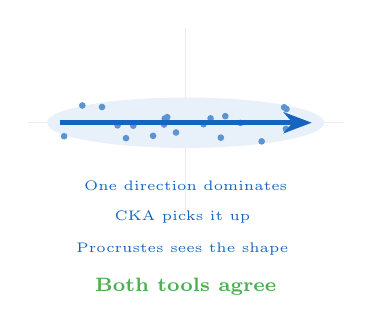
\begin{tikzpicture}[scale=0.8]
  \draw[neutral!20] (-2.5,0) -- (2.5,0);
  \draw[neutral!20] (0,-1.5) -- (0,1.5);

  % Elongated cloud along one axis
  \fill[dimlow!10] (0,0) ellipse (2.2 and 0.4);
  \foreach \i in {1,...,20} {
    \pgfmathsetmacro{\x}{2.0*rand}
    \pgfmathsetmacro{\y}{0.3*rand}
    \fill[dimlow!70] (\x,\y) circle (1.5pt);
  }
  \draw[dimlow,ultra thick,-{Stealth}] (-2,0) -- (2,0);

  \node[font=\tiny,dimlow,align=center] at (0,-1.0) {One direction dominates};
  \node[font=\tiny,dimlow,align=center] at (0,-1.5) {CKA picks it up $\checkmark$};
  \node[font=\tiny,dimlow,align=center] at (0,-2.0) {Procrustes sees the shape $\checkmark$};
  \node[font=\scriptsize,pass] at (0,-2.6) {\textbf{Both tools agree}};
\end{tikzpicture}
\end{column}
\begin{column}{0.5\textwidth}
\centering
\textbf{\textcolor{dimhigh}{High-dimensional region (MOs-type)}}

\vspace{0.3em}
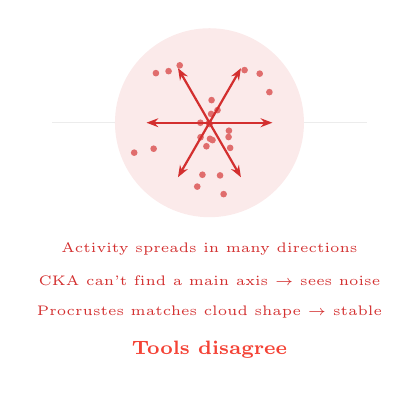
\begin{tikzpicture}[scale=0.8]
  \draw[neutral!20] (-2.5,0) -- (2.5,0);
  \draw[neutral!20] (0,-1.5) -- (0,1.5);

  % Spherical cloud — no dominant axis
  \fill[dimhigh!10] (0,0) circle (1.5);
  \foreach \i in {1,...,25} {
    \pgfmathsetmacro{\a}{360*rnd}
    \pgfmathsetmacro{\r}{1.3*rnd}
    \fill[dimhigh!70] ({(\r)*cos(\a)},{(\r)*sin(\a)}) circle (1.5pt);
  }
  % Multiple equal arrows
  \foreach \a in {0,60,...,300} {
    \draw[dimhigh,thick,-{Stealth[length=1.5mm]}] (0,0) -- ({1.0*cos(\a)},{1.0*sin(\a)});
  }

  \node[font=\tiny,dimhigh,align=center] at (0,-2.0) {Activity spreads in many directions};
  \node[font=\tiny,dimhigh,align=center] at (0,-2.5) {CKA can't find a main axis $\to$ sees noise};
  \node[font=\tiny,dimhigh,align=center] at (0,-3.0) {Procrustes matches cloud shape $\to$ stable};
  \node[font=\scriptsize,fail] at (0,-3.6) {\textbf{Tools disagree}};
\end{tikzpicture}
\end{column}
\end{columns}
\end{frame}

%% --- SLIDE: The anti-correlation — data ---
\begin{frame}{The data: CKA and Procrustes are anti-correlated}
\begin{columns}[T]
\begin{column}{0.68\textwidth}
\centering
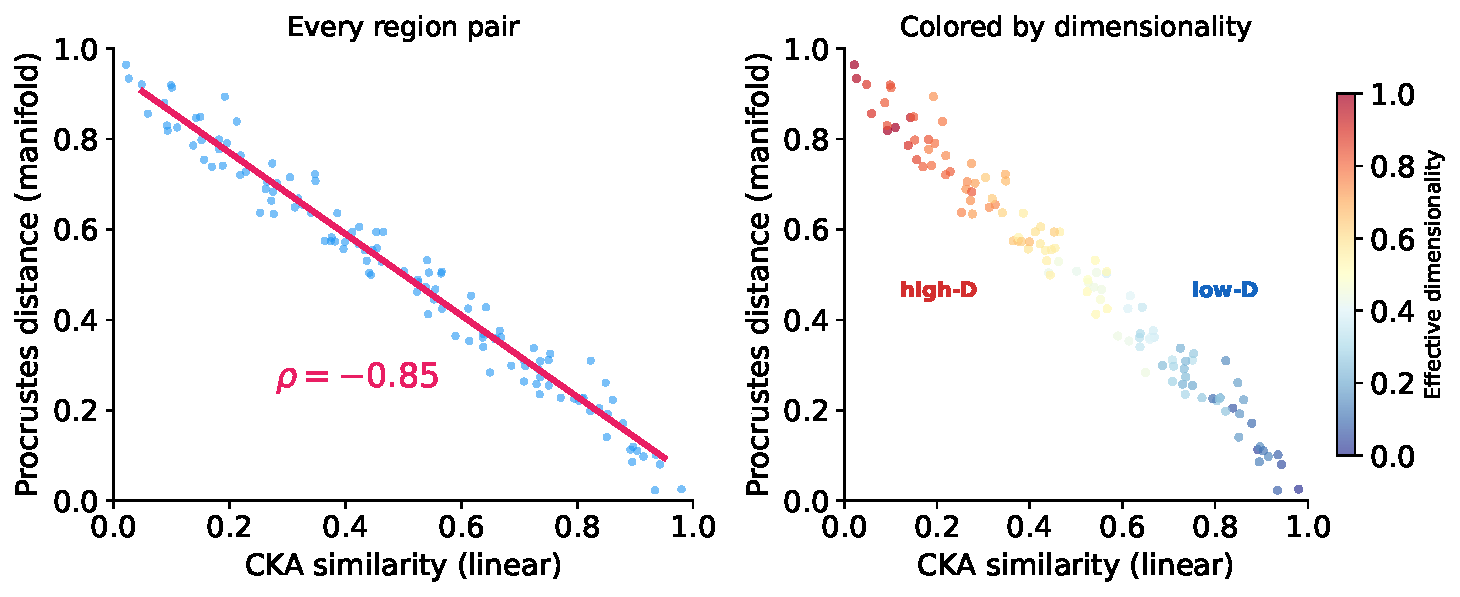
\includegraphics[width=\linewidth]{anticorrelation_scatter.pdf}
\end{column}
\begin{column}{0.30\textwidth}
\vspace{0.5em}
{\small Each dot is a pair of brain regions. The two tools rank them in \textbf{opposite order} (correlation $= -0.85$; $-1$ would be perfect reversal).}

\vspace{0.5em}
{\small \textbf{Why?} The right panel colors dots by how ``spread out'' the neural activity is. Blue dots (compact activity) make both tools agree. Red dots (diffuse activity) make them disagree.}

\vspace{0.5em}
{\small Once you account for this spread, the disagreement shrinks from $-0.85$ to $-0.31$.}

\vspace{0.5em}
{\small We first found this in 5 recording sessions, then confirmed it held across all 39.}

\vspace{0.5em}
{\small \textbf{Takeaway:} the tool you pick determines what you find.}
\end{column}
\end{columns}
\end{frame}

%% --- SLIDE: Eigenvalue spectra ---
\begin{frame}{What determines dimensionality?}
\centering
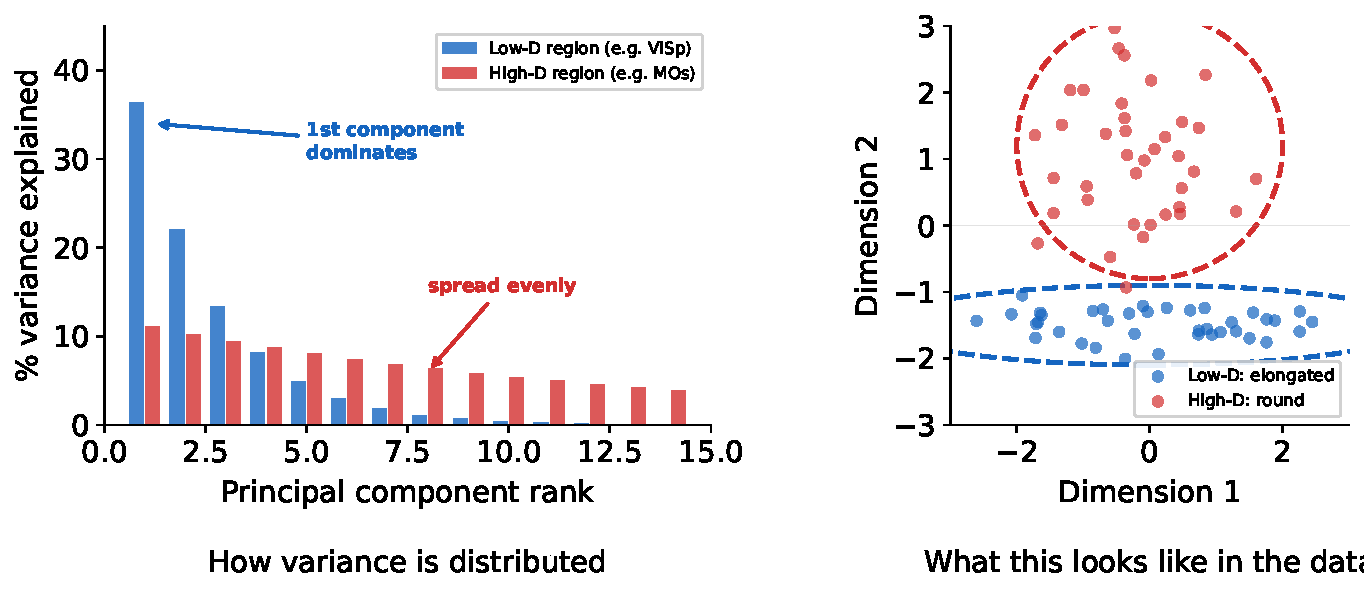
\includegraphics[width=0.85\linewidth]{eigenvalue_spectra.pdf}

\vspace{0.5em}
{\small Across all 73 regions, the \textbf{shape} of how variance falls off is nearly identical (correlation $0.94$ out of $1.0$). But \textbf{which neurons} carry the variance is completely different per region (correlation $0.09$, barely above zero). Same scaffolding, different content.}
\end{frame}

%% ============================================================
%% PART 3: MORE DESCRIPTIVE FINDINGS
%% ============================================================

%% --- SLIDE: Rotation ---
\begin{frame}{Every brain region rotates (but at very different speeds)}
\begin{columns}[T]
\begin{column}{0.42\textwidth}
\centering
{\small \textbf{What rotation means}}

\vspace{0.3em}
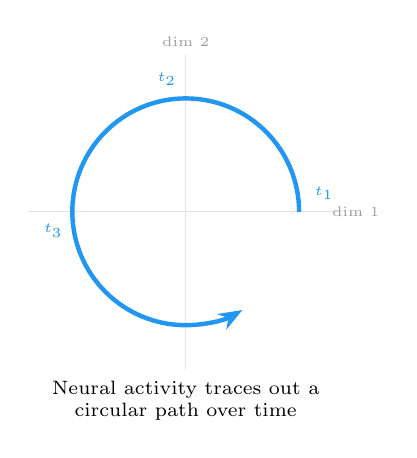
\begin{tikzpicture}[scale=0.8]
  \draw[neutral!30,thin] (-2.5,0) -- (2.5,0);
  \draw[neutral!30,thin] (0,-2.5) -- (0,2.5);
  \node[font=\tiny,neutral] at (2.7,0) {dim 1};
  \node[font=\tiny,neutral] at (0,2.7) {dim 2};
  \draw[evidence,ultra thick,-{Stealth[length=3mm]}]
    (1.8,0) arc[start angle=0, end angle=300, radius=1.8];
  \node[font=\tiny,evidence] at (2.2,0.3) {$t_1$};
  \node[font=\tiny,evidence] at (-0.3,2.1) {$t_2$};
  \node[font=\tiny,evidence] at (-2.1,-0.3) {$t_3$};
  \node[font=\scriptsize,align=center] at (0,-3) {Neural activity traces out a\\circular path over time};
\end{tikzpicture}
\end{column}
\begin{column}{0.56\textwidth}
\centering
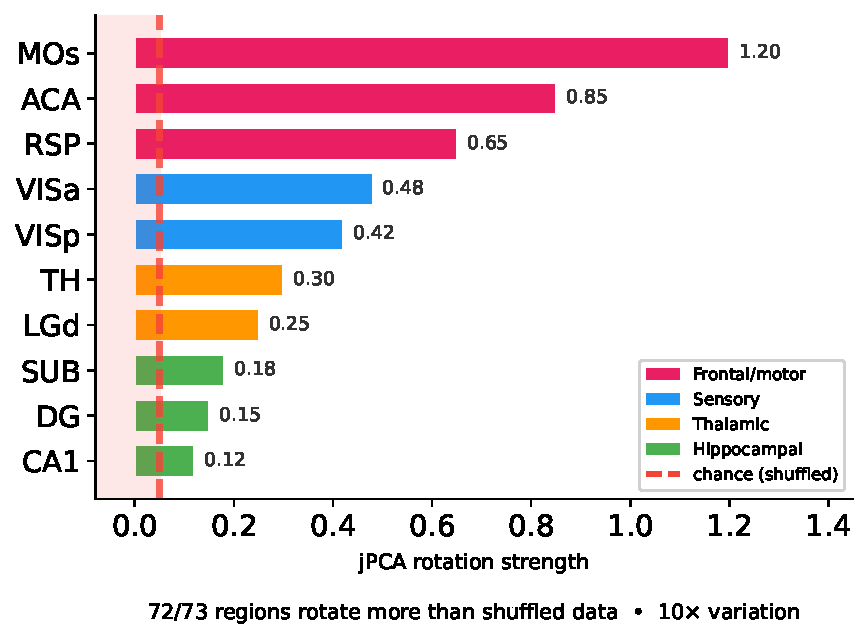
\includegraphics[width=\linewidth]{jpca_rotation.pdf}
\end{column}
\end{columns}
\end{frame}

%% --- SLIDE: Anatomy recovery (sanity check) ---
\begin{frame}{Sanity check: geometry tracks known anatomy}
\begin{columns}[T]
\begin{column}{0.5\textwidth}
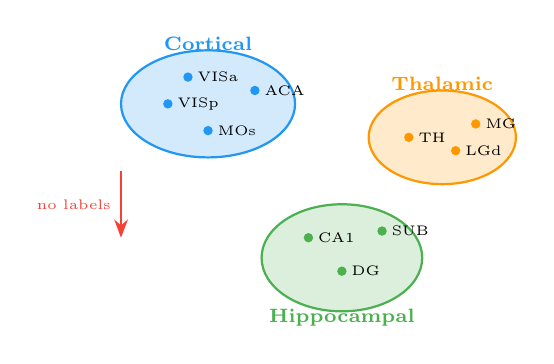
\begin{tikzpicture}[scale=0.85]
  \fill[evidence!20] (-1.5,2) ellipse (1.3 and 0.8);
  \draw[evidence,thick] (-1.5,2) ellipse (1.3 and 0.8);
  \node[evidence,font=\scriptsize\bfseries] at (-1.5,2.9) {Cortical};
  \foreach \name/\x/\y in {VISp/-2.1/2, MOs/-1.5/1.6, ACA/-0.8/2.2, VISa/-1.8/2.4} {
    \fill[evidence] (\x,\y) circle (2pt);
    \node[font=\tiny,right] at (\x,\y) {\name};
  }
  \fill[causal!20] (2,1.5) ellipse (1.1 and 0.7);
  \draw[causal,thick] (2,1.5) ellipse (1.1 and 0.7);
  \node[causal,font=\scriptsize\bfseries] at (2,2.3) {Thalamic};
  \foreach \name/\x/\y in {TH/1.5/1.5, LGd/2.2/1.3, MG/2.5/1.7} {
    \fill[causal] (\x,\y) circle (2pt);
    \node[font=\tiny,right] at (\x,\y) {\name};
  }
  \fill[geometry!20] (0.5,-0.3) ellipse (1.2 and 0.8);
  \draw[geometry,thick] (0.5,-0.3) ellipse (1.2 and 0.8);
  \node[geometry,font=\scriptsize\bfseries] at (0.5,-1.2) {Hippocampal};
  \foreach \name/\x/\y in {CA1/0/0, DG/0.5/-0.5, SUB/1.1/0.1} {
    \fill[geometry] (\x,\y) circle (2pt);
    \node[font=\tiny,right] at (\x,\y) {\name};
  }
  \draw[fail,thick,{Stealth}-] (-2.8,0) -- (-2.8,1) node[midway,left,font=\tiny,fail] {no labels};
\end{tikzpicture}
\end{column}
\begin{column}{0.48\textwidth}
{\small We grouped brain regions \emph{purely by how similar their neural activity looks}---no anatomy labels as input.}

\vspace{0.3em}
{\small \textbf{Result:} the algorithm found three groups matching the textbook cortical / thalamic / hippocampal division on its own.}

\vspace{0.3em}
{\small \textbf{Why this matters:} CKA is a general-purpose metric, not designed for neuroscience. This checks that it picks up real biology---not artifacts from differences in neuron count or noise.}

\vspace{0.3em}
{\small Same result within individual sessions and across animals.}
\end{column}
\end{columns}
\end{frame}

%% ============================================================
%% PART 4: CAUSAL INTERVENTIONS
%% ============================================================
\section{Is the geometry causal?}

%% --- SLIDE: Recap the task ---
\begin{frame}{Recap: what the mouse is doing}
\begin{columns}[T]
\begin{column}{0.5\textwidth}
\centering
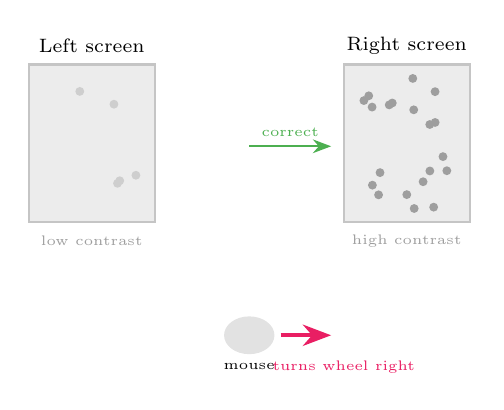
\begin{tikzpicture}[scale=0.8]
  % Left screen
  \fill[neutral!20] (-3.5,0) rectangle (-1.5,2.5);
  \draw[neutral!60,thick] (-3.5,0) rectangle (-1.5,2.5);
  \node[font=\scriptsize] at (-2.5,2.8) {Left screen};
  % Sparse dots = low contrast
  \foreach \i in {1,...,5} {
    \pgfmathsetmacro{\x}{-3.3+1.6*rnd}
    \pgfmathsetmacro{\y}{0.2+2.1*rnd}
    \fill[neutral!50] (\x,\y) circle (2pt);
  }
  \node[font=\tiny,neutral] at (-2.5,-0.3) {low contrast};

  % Right screen
  \fill[neutral!20] (1.5,0) rectangle (3.5,2.5);
  \draw[neutral!60,thick] (1.5,0) rectangle (3.5,2.5);
  \node[font=\scriptsize] at (2.5,2.8) {Right screen};
  % Dense dots = high contrast
  \foreach \i in {1,...,20} {
    \pgfmathsetmacro{\x}{1.7+1.6*rnd}
    \pgfmathsetmacro{\y}{0.2+2.1*rnd}
    \fill[neutral] (\x,\y) circle (2pt);
  }
  \node[font=\tiny,neutral] at (2.5,-0.3) {high contrast};

  % Mouse + wheel
  \fill[neutral!30] (0,-1.8) ellipse (0.4 and 0.3);
  \node[font=\tiny] at (0,-2.3) {mouse};
  \draw[choice,ultra thick,-{Stealth}] (0.5,-1.8) -- (1.3,-1.8);
  \node[choice,font=\tiny] at (1.5,-2.3) {turns wheel right};

  % Arrow showing correct choice
  \draw[pass,thick,-{Stealth}] (0,1.2) -- (1.3,1.2);
  \node[pass,font=\tiny,above] at (0.65,1.2) {correct};
\end{tikzpicture}
\end{column}
\begin{column}{0.48\textwidth}
\vspace{0.5em}
{\small The mouse sees two screens with random visual noise. One side has \textbf{higher contrast} (more visible dots). The mouse turns a wheel toward that side to get a reward.}

\vspace{0.3em}
{\small \textbf{``Evidence''} = which side has higher contrast. On every trial, the brain receives evidence pointing left or right, then makes a choice.}

\vspace{0.3em}
{\small \textbf{The question:} somewhere in the neural activity, there must be a signal carrying this evidence from sensory areas to the decision. We call it the ``evidence subspace.''}
\end{column}
\end{columns}
\end{frame}

%% --- SLIDE: The intervention ---
\begin{frame}{Testing causality: swap the evidence signal between trials}
\begin{columns}[T]
\begin{column}{0.55\textwidth}
{\small Showing that neural activity \emph{correlates} with a decision is easy. Showing it \emph{causes} the decision is hard.}

\vspace{0.3em}
{\small \textbf{Our test:} take two trials where the mouse saw opposite evidence:}
\begin{itemize}\setlength\itemsep{2pt}
  \item {\small Trial A: stronger on the \textbf{left} $\to$ mouse chose left}
  \item {\small Trial B: stronger on the \textbf{right} $\to$ mouse chose right}
\end{itemize}

\vspace{0.3em}
{\small Now \textbf{swap only the evidence dimensions} of their neural activity (leaving everything else untouched) and re-run the choice decoder.}

\vspace{0.3em}
{\small If the predicted choice flips, those dimensions \textbf{causally carry} the evidence signal.}

\vspace{0.3em}
{\small \textcolor{neutral}{Method: interchange intervention analysis, adapted from Geiger et al.\ 2024.}}
\end{column}
\begin{column}{0.42\textwidth}
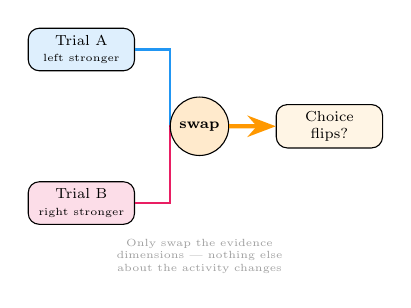
\begin{tikzpicture}[scale=0.75, every node/.style={transform shape},
  box/.style={draw,rounded corners,minimum width=1.8cm,minimum height=0.7cm,font=\scriptsize},
]
  \node[box,fill=evidence!15,align=center] (A) at (0,2.8) {Trial A\\{\tiny left stronger}};
  \node[box,fill=choice!15,align=center] (B) at (0,0.2) {Trial B\\{\tiny right stronger}};

  \draw[evidence,thick,-{Stealth}] (A.east) -- ++(0.6,0) |- (2,1.5);
  \draw[choice,thick,-{Stealth}] (B.east) -- ++(0.6,0) |- (2,1.5);

  \node[draw,circle,fill=causal!20,minimum size=0.9cm,font=\scriptsize\bfseries] (swap) at (2,1.5) {swap};
  \node[box,fill=causal!10,align=center] (out) at (4.2,1.5) {Choice\\flips?};
  \draw[-{Stealth},ultra thick,causal] (swap) -- (out);

  \node[font=\tiny,neutral,text width=3cm,align=center] at (2,-0.7) {Only swap the evidence\\dimensions --- nothing else\\about the activity changes};
\end{tikzpicture}
\end{column}
\end{columns}
\end{frame}

%% --- SLIDE: IIA results with baselines ---
\begin{frame}{Result: swapping evidence dimensions flips choices}
\begin{columns}[T]
\begin{column}{0.5\textwidth}
\centering
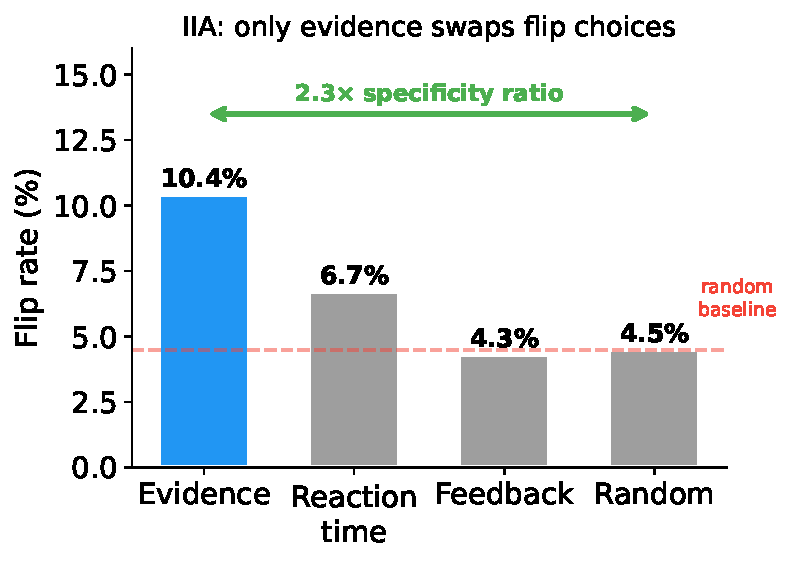
\includegraphics[width=\linewidth]{iia_bars.pdf}
\end{column}
\begin{column}{0.48\textwidth}
{\small \textbf{What each bar means:}}
\begin{itemize}
  \item \textbf{\textcolor{evidence}{Evidence}}: swap the subspace that encodes which side has higher contrast
  \item \textbf{RT}: swap the subspace encoding reaction time
  \item \textbf{Feedback}: swap correct/error encoding
  \item \textbf{Random}: swap a random subspace
\end{itemize}

\vspace{0.5em}
\textbf{Key numbers:}\\
Evidence flip rate: \textbf{10.4\%}\\
Random baseline: \textbf{4.5\%}\\
Ratio: \textbf{2.3$\times$} ($p < 0.001$)

\vspace{0.5em}
{\small The effect is modest in absolute terms. But only the evidence axis produces it---not RT, not feedback, not random. That specificity is what makes it causal.}
\end{column}
\end{columns}
\end{frame}

%% --- SLIDE: Sufficiency ---
\begin{frame}{The evidence subspace is sufficient (and denoises)}
\begin{columns}[T]
\begin{column}{0.5\textwidth}
\centering
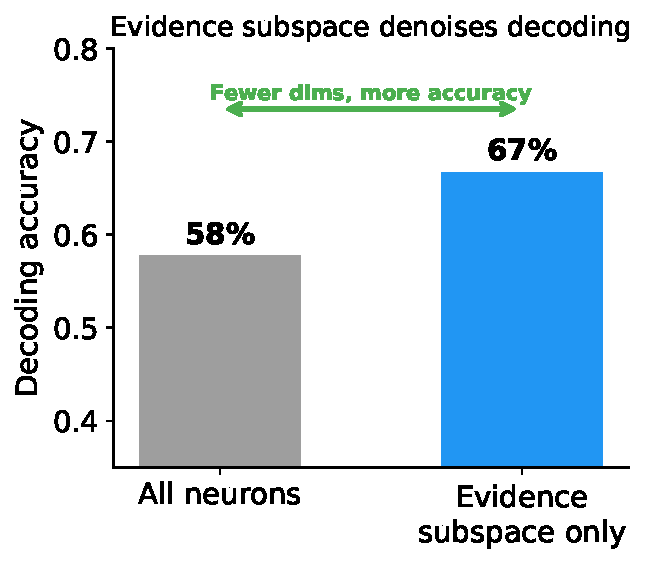
\includegraphics[width=0.85\linewidth]{sufficiency.pdf}
\end{column}
\begin{column}{0.48\textwidth}
If we restrict a classifier to \emph{only} the evidence subspace dimensions, it decodes choice \textbf{better} than using all neurons.

\vspace{0.5em}
\textbf{Why?} The evidence subspace acts as a denoiser---it strips away irrelevant neural variation that confuses the classifier.

\vspace{0.8em}
\textbf{20 of 24 regions pass} the $\geq 0.70$ recovery threshold.

\vspace{0.5em}
{\small The 4 failures are all high-dimensional regions where subspace estimation is harder.}

\vspace{0.5em}
{\small Together with IIA (necessity), this establishes the evidence subspace as a \textbf{causal mediator} of choice.}
\end{column}
\end{columns}
\end{frame}

%% --- SLIDE: Four methods agree ---
\begin{frame}{Four different intervention methods agree}
\begin{columns}[T]
\begin{column}{0.5\textwidth}
\centering
{\small We tested \textbf{four different ways} to intervene:}

\vspace{0.5em}
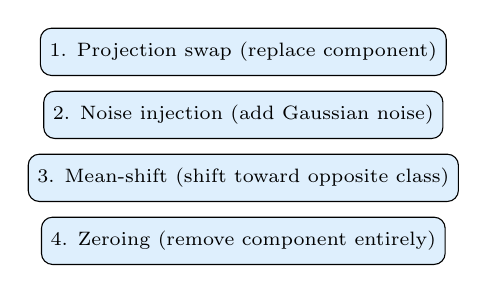
\begin{tikzpicture}[
  meth/.style={draw,rounded corners,fill=#1!15,minimum width=4cm,
    minimum height=0.6cm,font=\scriptsize},
]
  \node[meth=evidence] at (0,2.5) {1. Projection swap (replace component)};
  \node[meth=evidence] at (0,1.7) {2. Noise injection (add Gaussian noise)};
  \node[meth=evidence] at (0,0.9) {3. Mean-shift (shift toward opposite class)};
  \node[meth=evidence] at (0,0.1) {4. Zeroing (remove component entirely)};
\end{tikzpicture}

\vspace{0.5em}
{\small These are mathematically different operations. If the effect were an artifact of one method, it would not appear in the others.}
\end{column}
\begin{column}{0.48\textwidth}
\centering
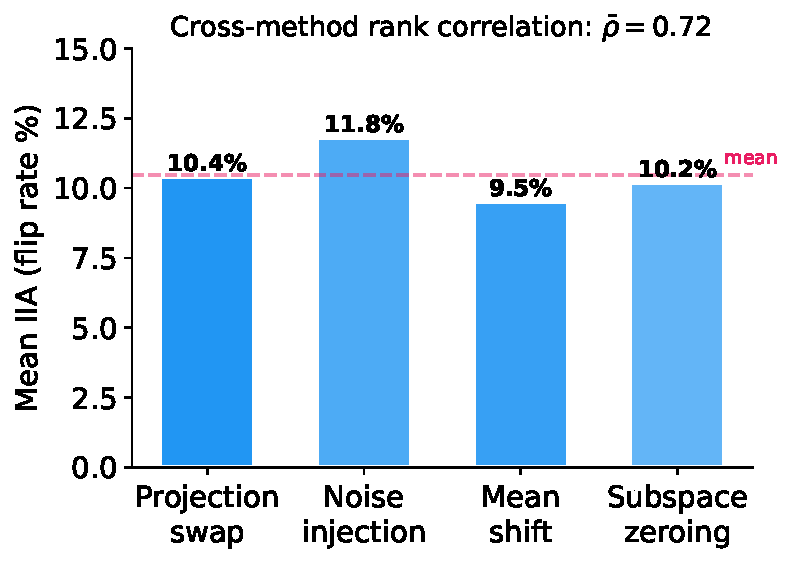
\includegraphics[width=\linewidth]{multi_method.pdf}

\vspace{0.3em}
{\small Regions that show high IIA with one method show high IIA with all four. The effect is method-invariant.}
\end{column}
\end{columns}
\end{frame}

%% ============================================================
%% PART 5: VALIDATION
%% ============================================================
\section{Did we fool ourselves?}

%% --- SLIDE: What could go wrong ---
\begin{frame}{What could go wrong?}
Before trusting these results, we need to rule out simpler explanations:

\vspace{0.5em}
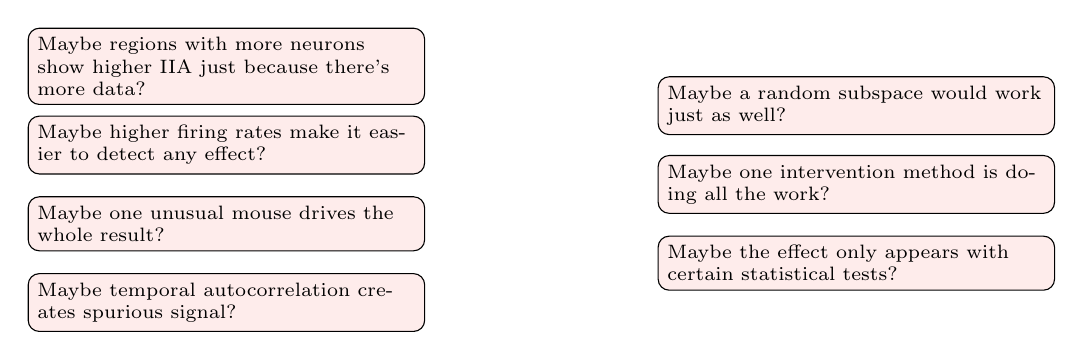
\begin{tikzpicture}[
  concern/.style={draw,rounded corners,fill=#1!10,minimum width=5cm,
    minimum height=0.6cm,font=\scriptsize,text width=4.8cm},
]
  \node[concern=fail] (c1) at (0,3) {Maybe regions with more neurons show higher IIA just because there's more data?};
  \node[concern=fail] (c2) at (0,2) {Maybe higher firing rates make it easier to detect any effect?};
  \node[concern=fail] (c3) at (0,1) {Maybe one unusual mouse drives the whole result?};
  \node[concern=fail] (c4) at (0,0) {Maybe temporal autocorrelation creates spurious signal?};
  \node[concern=fail] (c5) at (8,2.5) {Maybe a random subspace would work just as well?};
  \node[concern=fail] (c6) at (8,1.5) {Maybe one intervention method is doing all the work?};
  \node[concern=fail] (c7) at (8,0.5) {Maybe the effect only appears with certain statistical tests?};
\end{tikzpicture}

\vspace{0.8em}
We tested each of these. The framework comes from philosophy of science: validity criteria from Craver (2007), Shallice (1988), and Mayo (2018).
\end{frame}

%% --- SLIDE: Confound control ---
\begin{frame}{Confound control: what doesn't explain the effect}
\begin{columns}[T]
\begin{column}{0.5\textwidth}
\centering
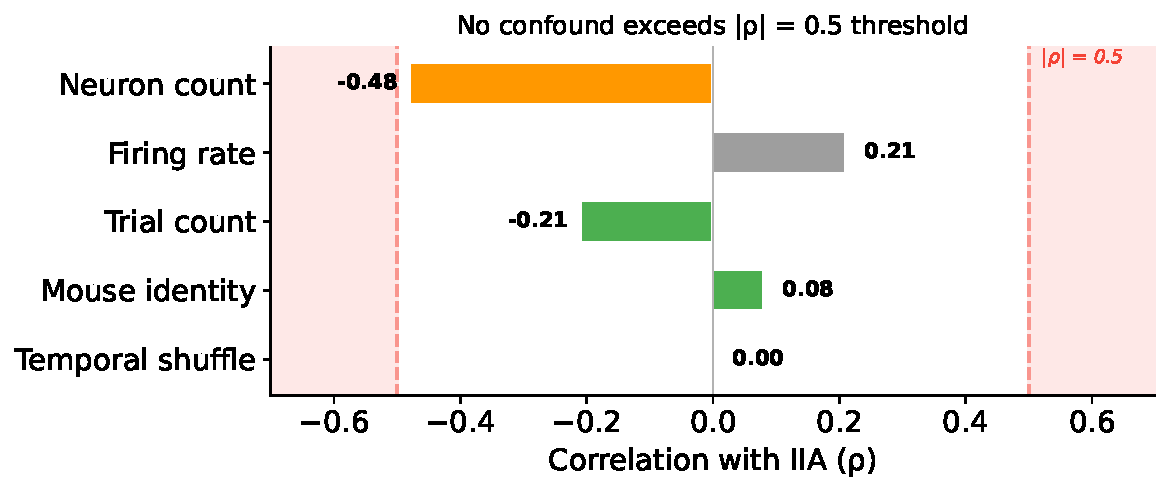
\includegraphics[width=\linewidth]{confounds.pdf}
\end{column}
\begin{column}{0.48\textwidth}
{\small ($\rho$ = correlation: 0 means no relationship, $\pm$1 means perfect; $|\rho| > 0.5$ is our danger zone.)}

\vspace{0.3em}
\textbf{Clear passes:}
\begin{itemize}\setlength\itemsep{1pt}
  \item Temporal shuffle: $\rho = 0.001$ \\
    {\small (scrambling time within trials doesn't change the effect --- it's not a timing artifact)}
  \item Mouse identity: $\rho = 0.08$ \\
    {\small (no single mouse drives the result)}
  \item Trial count: $\rho = -0.21$
  \item Firing rate: $\rho = 0.21$
\end{itemize}

\vspace{0.3em}
\textbf{Near-miss:}
\begin{itemize}\setlength\itemsep{1pt}
  \item Neuron count: $\rho = -0.48$ \\
    {\small Close to the line. Regions with fewer recorded neurons show slightly higher effects. Flagged in limitations.}
\end{itemize}
\end{column}
\end{columns}
\end{frame}

%% --- SLIDE: Graded response ---
\begin{frame}{Graded response: remove dimensions one at a time}
\begin{columns}[T]
\begin{column}{0.55\textwidth}
\centering
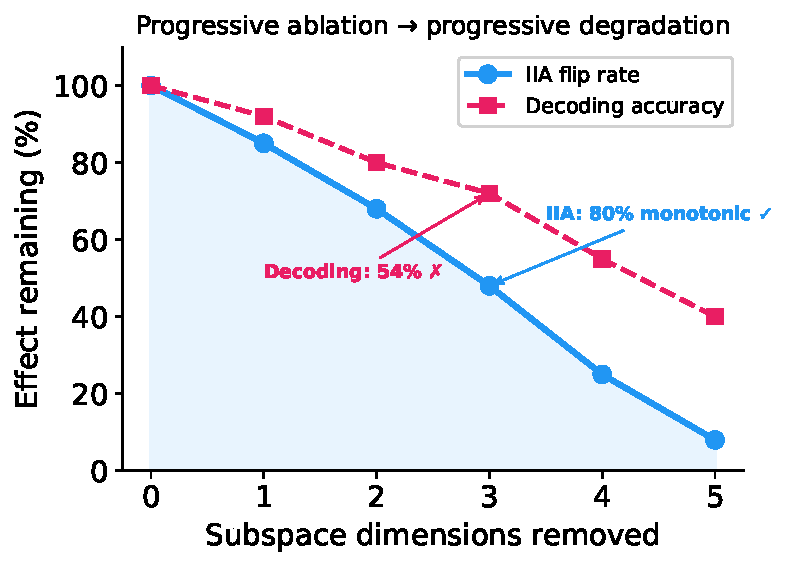
\includegraphics[width=\linewidth]{graded_response.pdf}
\end{column}
\begin{column}{0.43\textwidth}
\textbf{IIA (flip rate):} monotonic dose-response in \textbf{80\%} of regions {\small $\checkmark$}

\vspace{0.5em}
\textbf{Decoding accuracy:} monotonic in only \textbf{54\%} of regions {\small $\times$}

\vspace{0.5em}
{\small The IIA (causal) measure shows clean dose-response. The decoding (correlational) measure is less clean---some regions have redundant coding where removing one dimension shifts load to others.}

\vspace{0.5em}
{\small \textcolor{partial}{\textbf{Mixed:}} IIA passes, ablation fails. The causal effect is graded; the correlational proxy is not.}
\end{column}
\end{columns}
\end{frame}

%% --- SLIDE: Novel predictions ---
\begin{frame}{Novel predictions: what geometry tells us that we didn't know}
\begin{columns}[T]
\begin{column}{0.5\textwidth}
\textbf{Geometric type predicts decoder choice}\\[0.3em]
{\small If you know whether a brain region has ``linear'' or ``manifold'' geometry, you can predict which statistical decoder (LDA vs.\ kNN) will work better---without ever training on decoding data.}

\vspace{0.3em}
\centering {\small correlation $= -0.51$, highly significant ($p = 0.0002$, 50 regions)}

\vspace{0.8em}
\textbf{Causal abstraction}\\[0.3em]
{\small Regions with stronger low-dimensional structure route evidence to choice more efficiently (moderate effect).}

\vspace{0.3em}
\centering {\small correlation $= 0.29$, significant ($p = 0.014$)}
\end{column}
\begin{column}{0.48\textwidth}
\textbf{Allen Atlas: an honest null}\\[0.3em]
{\small We tested whether anatomical wiring (from the Allen Mouse Brain Atlas) predicts which regions show strong causal evidence routing.}

\vspace{0.3em}
\centering {\small correlation $= 0.03$, not significant ($p = 0.65$)}

\vspace{0.5em}
{\small \textbf{It doesn't.} Physical wiring between brain regions does not predict which ones causally carry evidence. The geometry we found captures something that pure anatomy misses.}

\vspace{0.8em}
{\small We report this null alongside the positive results. Three predictions made: two confirmed, one null.}
\end{column}
\end{columns}
\end{frame}

%% --- SLIDE: Validity scorecard ---
\begin{frame}{Validity scorecard}
{\small
\begin{tabular}{lp{6.5cm}c}
\toprule
\textbf{Criterion} & \textbf{What we tested} & \textbf{Status} \\
\midrule
\textbf{Necessity} & Swapping evidence subspace flips choice (2.3$\times$ above random) & \textcolor{pass}{\textbf{Pass}} \\
\textbf{Sufficiency} & Evidence subspace alone decodes better than full activity (1.16$\times$) & \textcolor{pass}{\textbf{Pass}} \\
\textbf{Specificity} & Only evidence axis flips; RT, feedback, random do not & \textcolor{pass}{\textbf{Pass}} \\
\textbf{Method invariance} & 4 intervention types agree (avg.\ correlation $0.72$) & \textcolor{pass}{\textbf{Pass}} \\
\textbf{Confound control} & No confound above $0.5$ threshold; neuron count $= 0.48$ (near-miss) & \textcolor{partial}{\textbf{Partial}} \\
\textbf{Double dissociation} & Evidence $\perp$ RT subspaces: 18\% dissociation rate & \textcolor{partial}{\textbf{Partial}} \\
\textbf{Cross-dataset} & IBL replication in progress & \textcolor{fail}{\textbf{Not yet}} \\
\bottomrule
\end{tabular}
}

\vspace{0.6em}
{\small Criteria adapted from Craver (2007), Mayo (2018), and Shallice (1988). We defined these before running the experiments, not after seeing the results.}
\end{frame}

%% ============================================================
%% PART 6: WHAT THIS MEANS
%% ============================================================
\section{What this means}

\begin{frame}{Summary: what we found and what it means}
\begin{columns}[T]
\begin{column}{0.5\textwidth}
\textbf{Descriptive findings:}
\begin{enumerate}
  \item Linear and manifold tools anti-correlate ($-0.85$); dimensionality explains why
  \item Variance structure is universal ($0.94$); neural content is not ($0.09$)
  \item Rotation everywhere (72/73), but 10$\times$ variation by region type
  \item Geometry clusters match anatomy (sanity check)
\end{enumerate}
\end{column}
\begin{column}{0.48\textwidth}
\textbf{Causal findings:}
\begin{enumerate}
  \setcounter{enumi}{4}
  \item Evidence subspace causally mediates choice (IIA, 10.4\% vs 4.5\% baseline)
  \item Effect is specific to evidence (not RT, feedback, random)
  \item Effect holds across 4 intervention methods (avg.\ correlation $0.72$)
  \item Evidence subspace denoises decoding (recovery 1.16)
\end{enumerate}
\end{column}
\end{columns}

\vspace{0.8em}
\textbf{The punchline:} Neural geometry is not metric-neutral---the tool you choose determines what you find, and dimensionality tells you which tool to trust. The causal structure we identify is modest but robust and specific.
\end{frame}

%% --- SLIDE: Limitations ---
\begin{frame}{Honest limitations}
\begin{columns}[T]
\begin{column}{0.5\textwidth}
\textbf{What limits these conclusions:}
\begin{itemize}
  \item \textbf{One dataset} (Steinmetz 2019)---needs replication
  \item \textbf{Binary task only}---unclear if geometry generalizes to richer tasks
  \item \textbf{Modest effect sizes}: 10.4\% flip rate (baseline 4.5\%)
  \item \textbf{Neuron count near-miss}: correlation $-0.48$
  \item \textbf{Double dissociation partial}: only 18\% rate
  \item \textbf{Exploratory}: no preregistration
\end{itemize}
\end{column}
\begin{column}{0.48\textwidth}
\textbf{What we're doing about it:}
\begin{itemize}
  \item IBL cross-dataset replication (in progress)
  \item Zatka-Haas optogenetic validation (silencing data downloaded)
  \item Multi-task generalization
  \item Dimensionality correction for neuron count
  \item Preregistered hypotheses for replication
\end{itemize}

\vspace{0.5em}
{\small We think reporting limitations this explicitly is itself unusual in the field, and worth doing.}
\end{column}
\end{columns}
\end{frame}

%% --- SLIDE: Intellectual grounding ---
\begin{frame}{Intellectual grounding}
This work draws on ideas from three research traditions:

\vspace{0.5em}
\begin{itemize}
  \item \textbf{Structured representation learning} (Esmaeili et al.\ 2019; Opper et al.\ 2023; ICML 2025)---explicit structural priors improve identifiability of learned representations. Our dimensionality-based metric taxonomy is an inductive bias argument: the right prior should reflect the data's geometric structure.
  \item \textbf{Relational causal models} (Maier et al.\ 2013; Arbour et al.\ 2016)---brain regions interact as a network, not as independent samples. Standard causal inference tools need adaptation for this.
  \item \textbf{Dynamical systems in neuroscience} (Sussillo \& Barak 2013; Vyas et al.\ 2020)---the connection between network dynamics and computational capacity. Our rotation findings connect to this tradition.
\end{itemize}

\vspace{0.5em}
Validity framework from philosophy of science (Mayo 2018, Craver 2007, Shallice 1988) and causal inference (Pearl \& Bareinboim 2011, Woodward 2003).
\end{frame}

%% --- SLIDE: Closing ---
\begin{frame}[standout]
  Code \& results: {\small [ZENODO DOI / GITHUB URL]}

  \vspace{1em}
  Neural geometry is not metric-neutral.\\[0.3em]
  The tool determines the finding.\\[0.3em]
  Dimensionality tells you which tool to trust.
\end{frame}

\end{document}
